\chapter{Appendices}

Appendices include additional graphs presenting the results of focus analysis.

\section{Yearly Focus}

This section presents four charts for yearly focus (\autoref{fig:yearly_2014-15}, \autoref{fig:yearly_2016-17}). It is visible that \textit{good developers} display higher yearly focus than \textit{bad developers}. However, the difference is quite small and it decreases with years.

\begin{figure}[htpb]
  \centering
  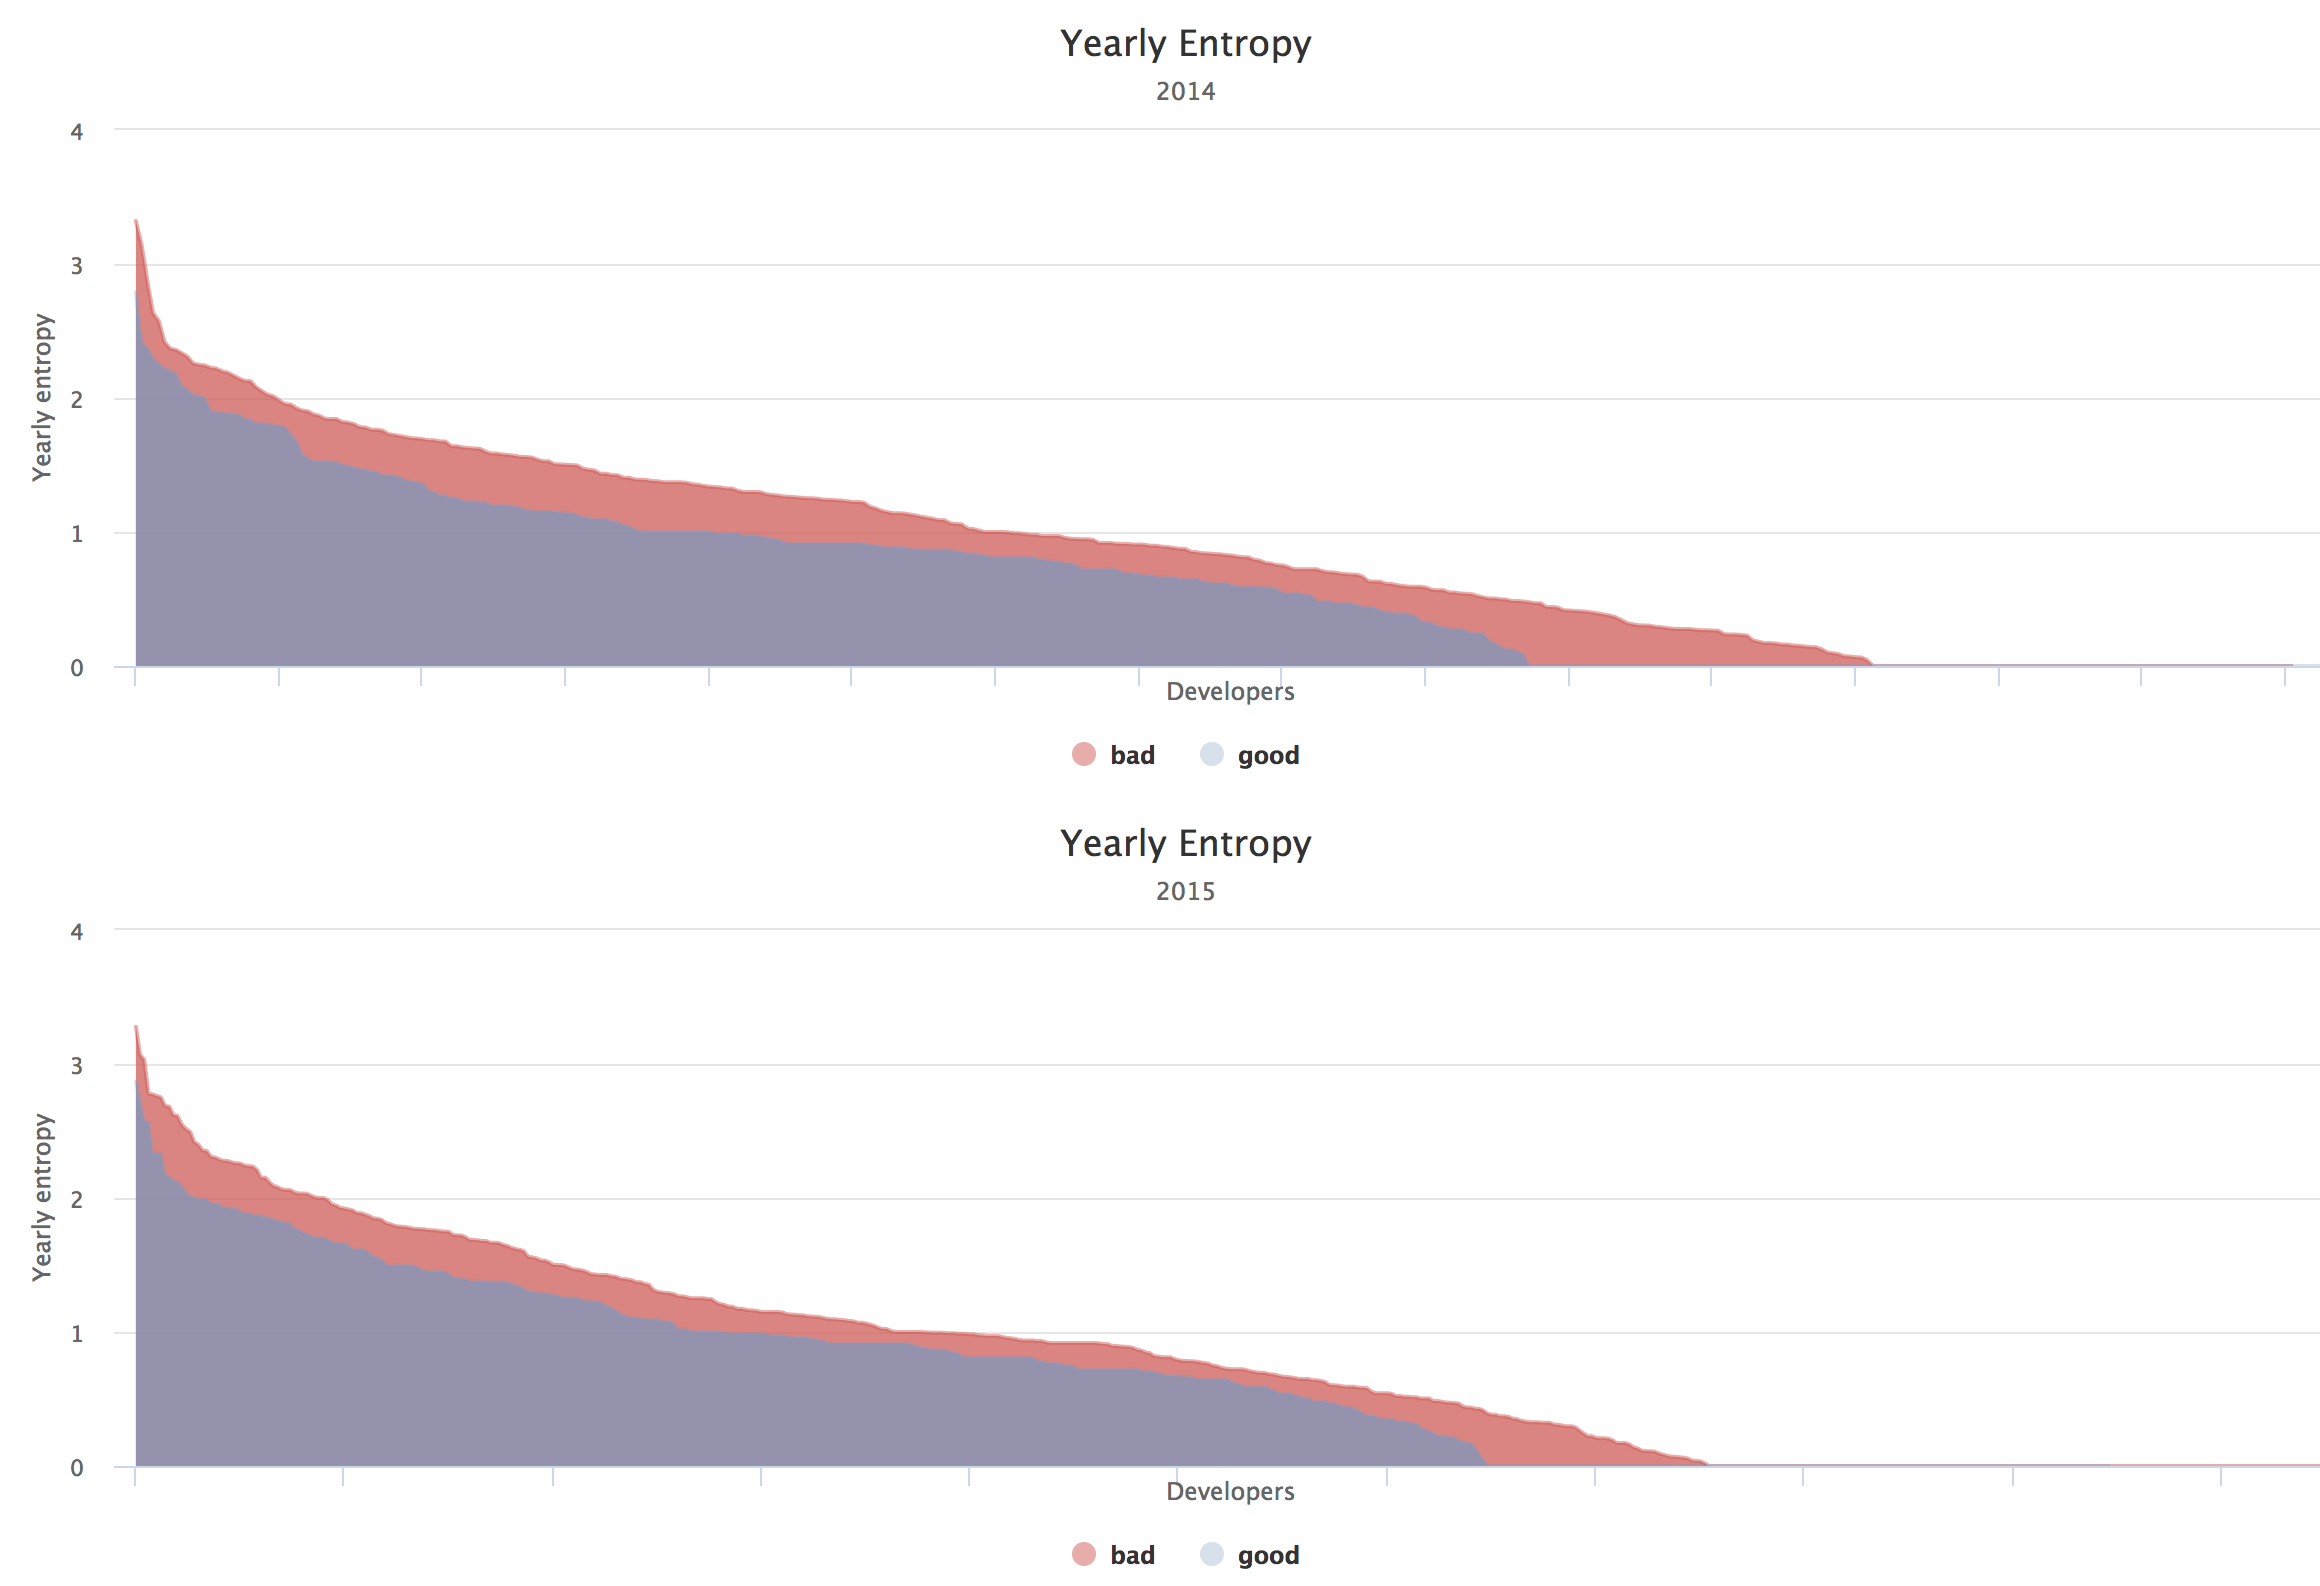
\includegraphics[width=1\textwidth]{figures/yearly_2014-15}
  \caption[Yearly Focus Chart for 2014 and 2015]{Yearly entropy values for \textit{good} and \textit{bad developers} displayed as overlapping area charts for years 2014 and 2015. Even on the yearly basis the good developers are more focused, although the difference is much less visible than with daily analysis. } \label{fig:yearly_2014-15}
\end{figure}

\begin{figure}[htpb]
  \centering
  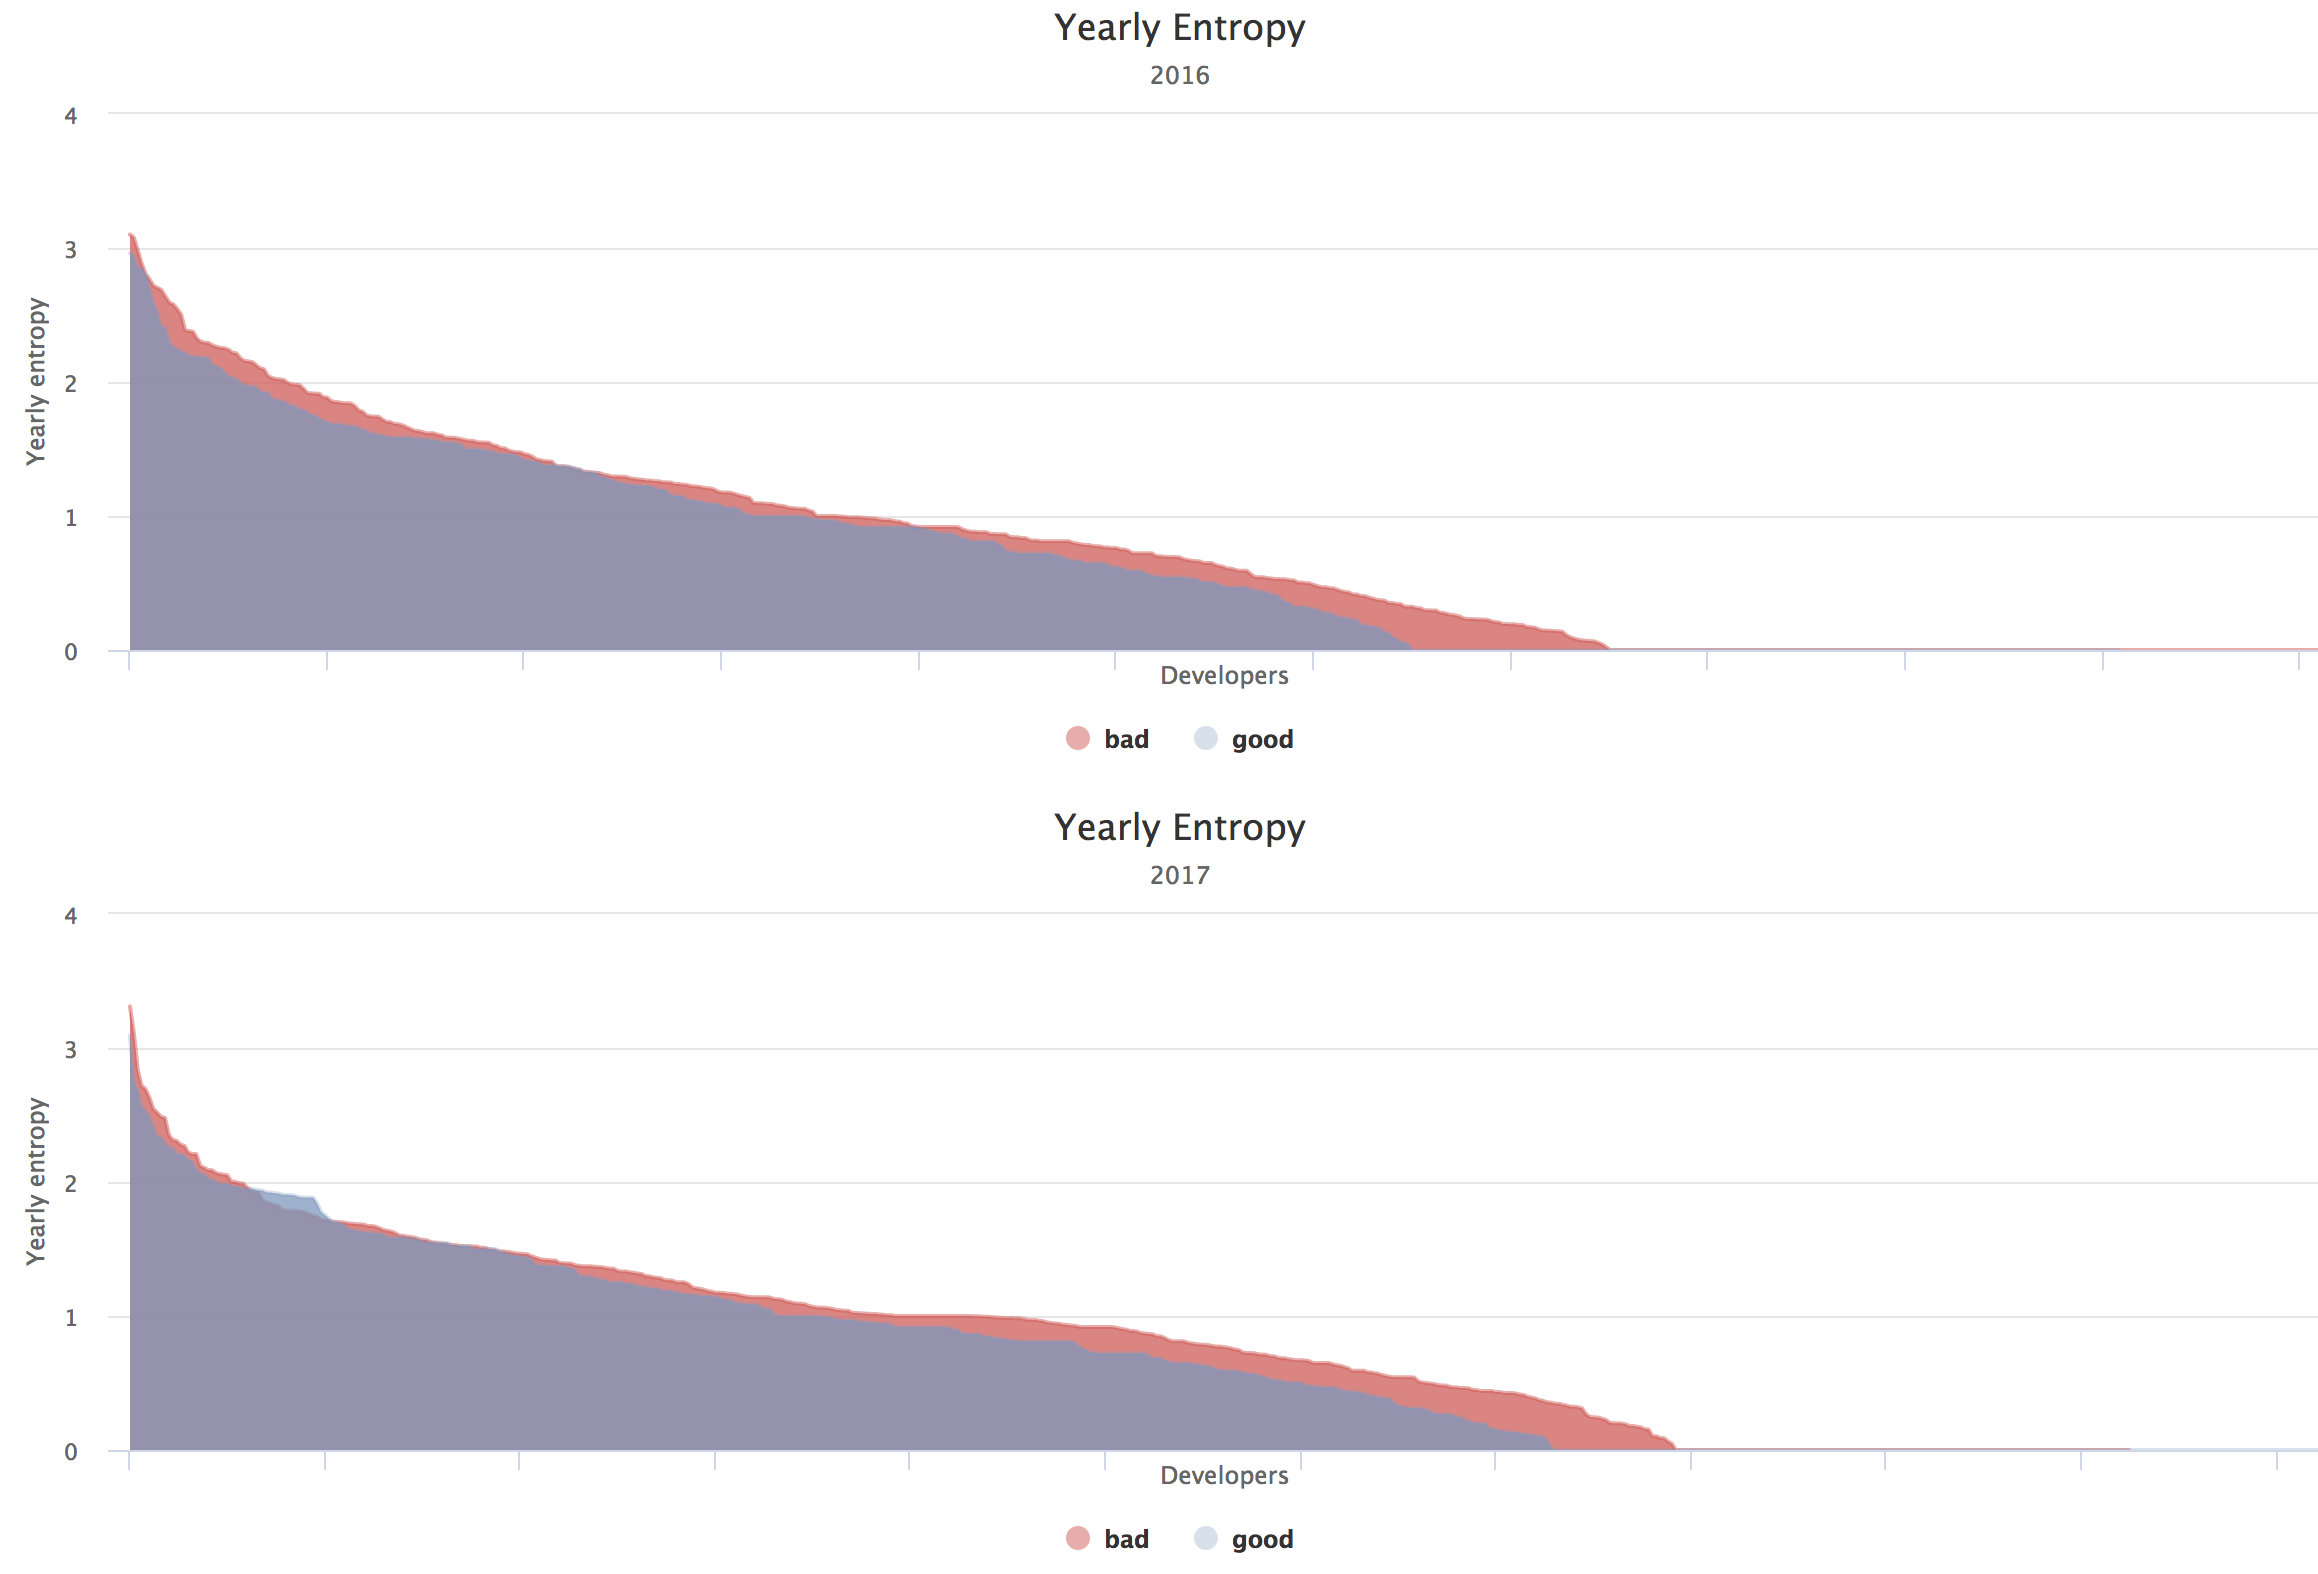
\includegraphics[width=1\textwidth]{figures/yearly_2016-17}
  \caption[Yearly Focus Chart for 2016 and 2017]{Yearly entropy values for \textit{good} and \textit{bad developers} displayed as overlapping area charts for years 2016 and 2017. Even on the yearly basis the good developers are more focused, although the difference is much less visible than with daily analysis. It is visible that the difference between \textit{good} and \textit{bad developers} gets smaller over years. } \label{fig:yearly_2016-17}
\end{figure}

\section{Focus For The Most Popular Extensions}

This section contains charts presenting the focus for each of ten most popular extensions. It is visible that \textit{good developers} are more focused on all but one extension. Ruby files seem to receive the same amount of focus from \textit{good} and \textit{bad developers} alike. Most of the extensions are related to coding, besides .txt, .md which are related to documentation and .lock which is a program file that developers do not write directly into.

\begin{figure}[htpb]
  \centering
  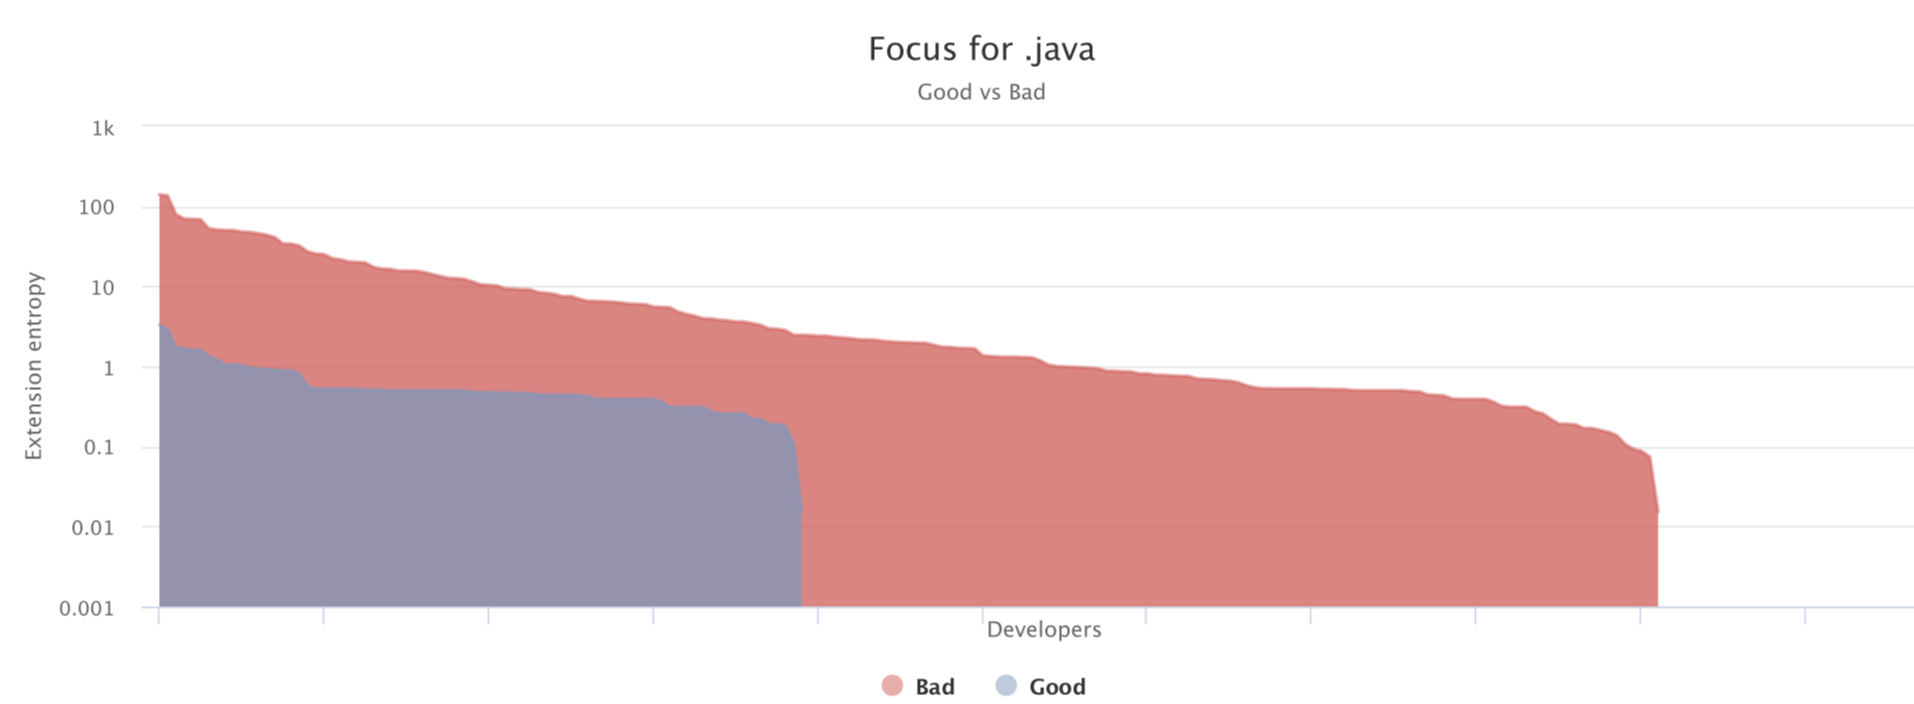
\includegraphics[width=1\textwidth]{figures/java_log}
  \caption[Focus Chart for .java]{Clearly \textit{good developers} focus more on .java extensions since the entropy levels are lower. This chart also shows that there are more \textit{bad developers} working on this extension.} \label{fig:java_log_appendix}
\end{figure}

\begin{figure}[htpb]
  \centering
  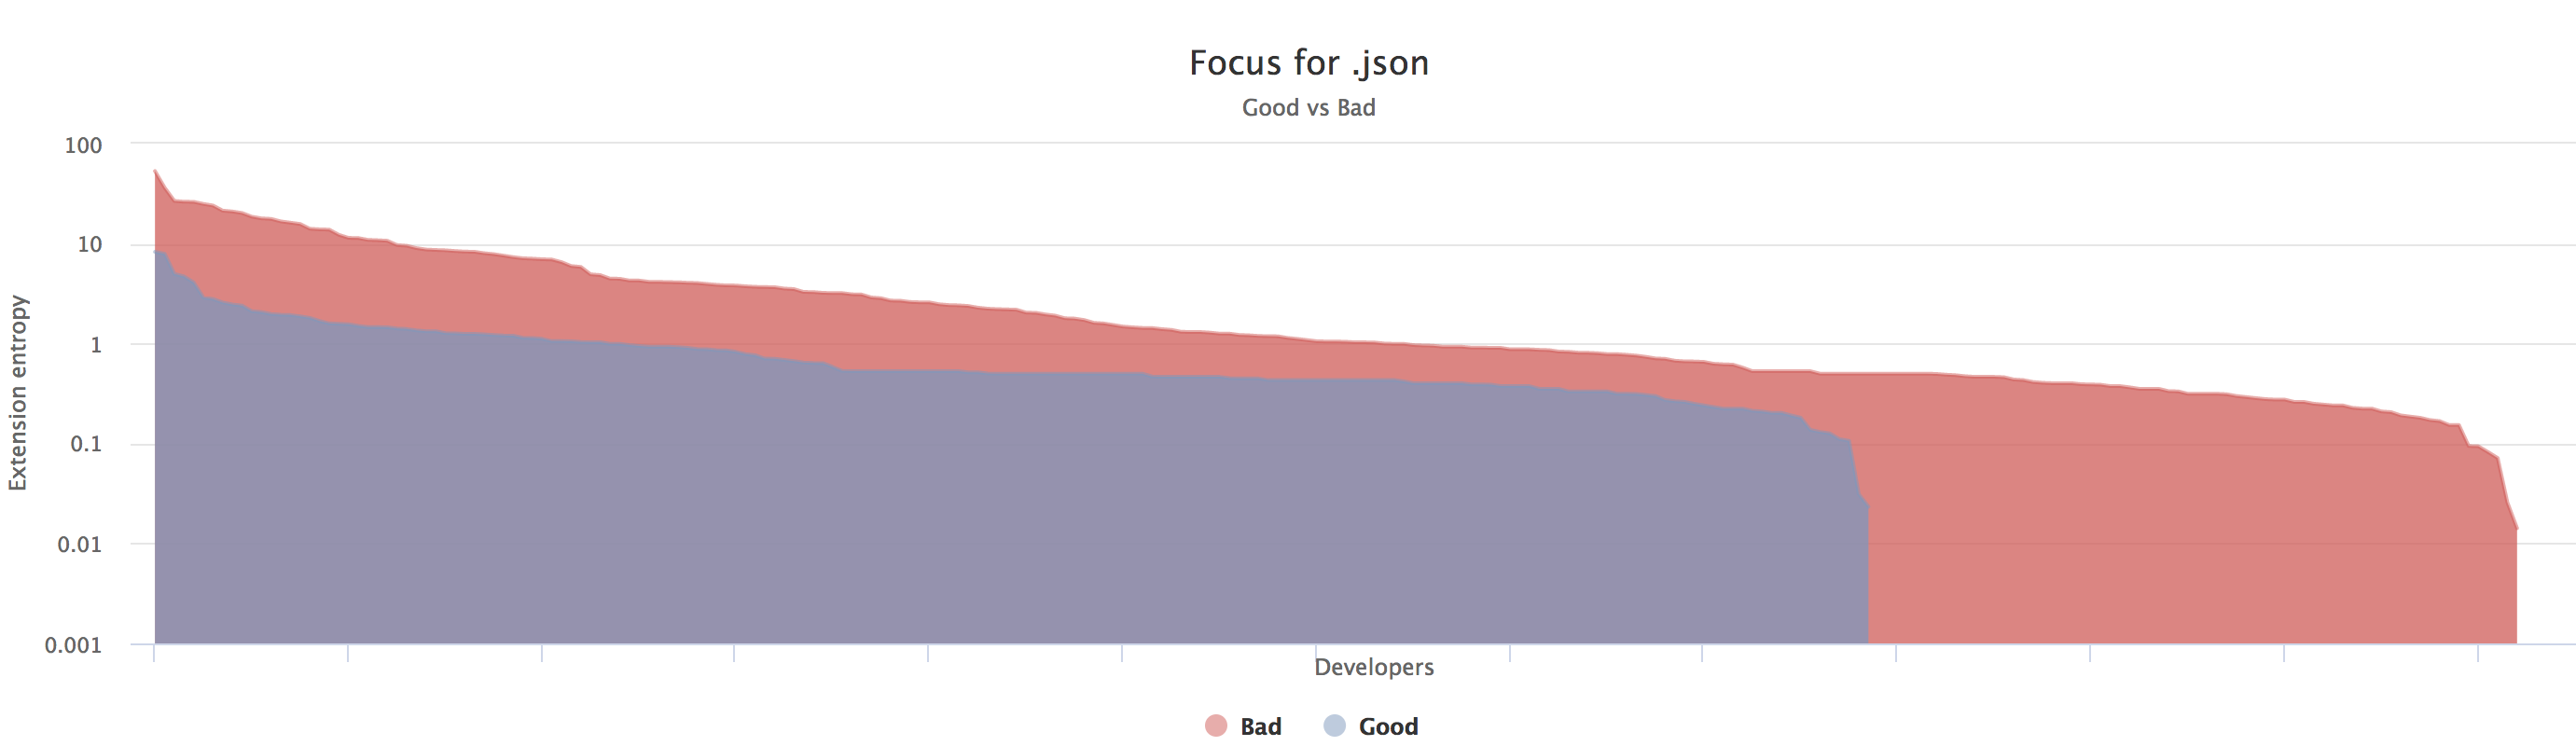
\includegraphics[width=1\textwidth]{figures/json_log}
  \caption[Focus Chart for .json]{Clearly \textit{good developers} focus more on .json extensions since the entropy levels are lower. This chart also shows that there are more \textit{bad developers} working on this extension.} \label{fig:json_log_appendix}
\end{figure}

\begin{figure}[htpb]
  \centering
  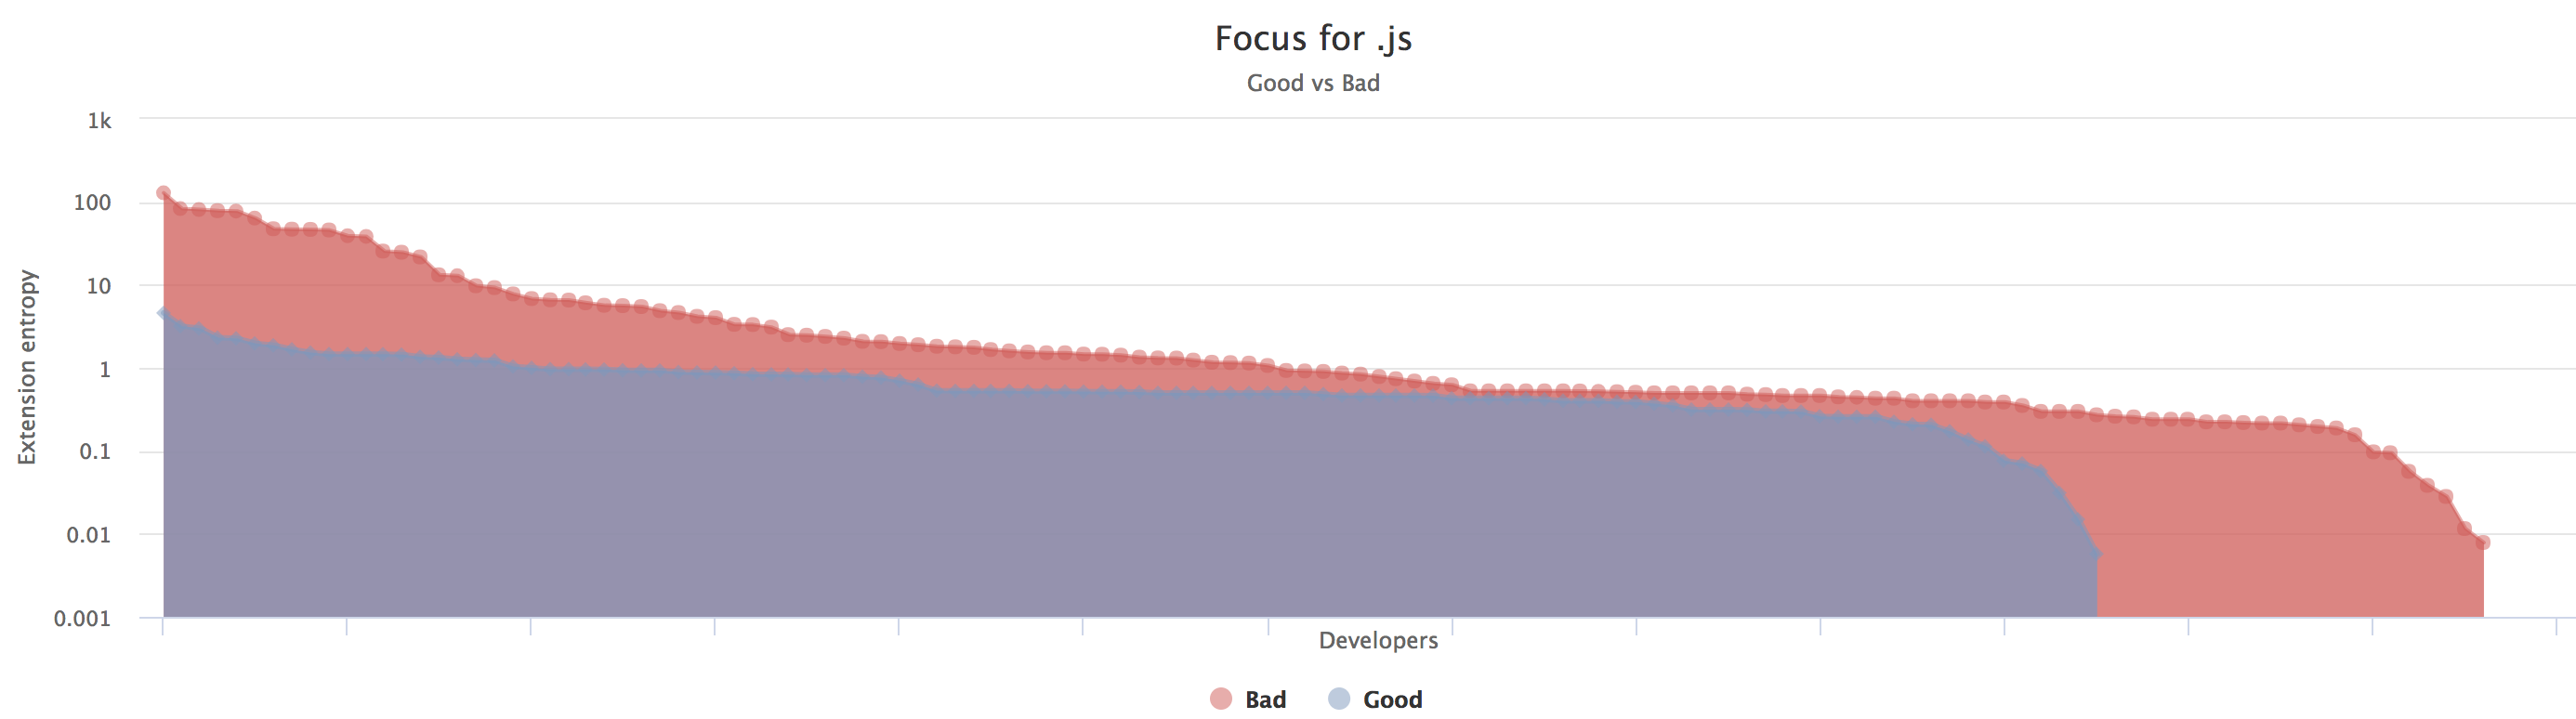
\includegraphics[width=1\textwidth]{figures/js_log}
  \caption[Focus Chart for .js]{Clearly \textit{good developers} focus more on .js extensions since the entropy levels are lower. This chart also shows that there are more \textit{bad developers} working on this extension.} \label{fig:js_log_appendix}
\end{figure}

\begin{figure}[htpb]
  \centering
  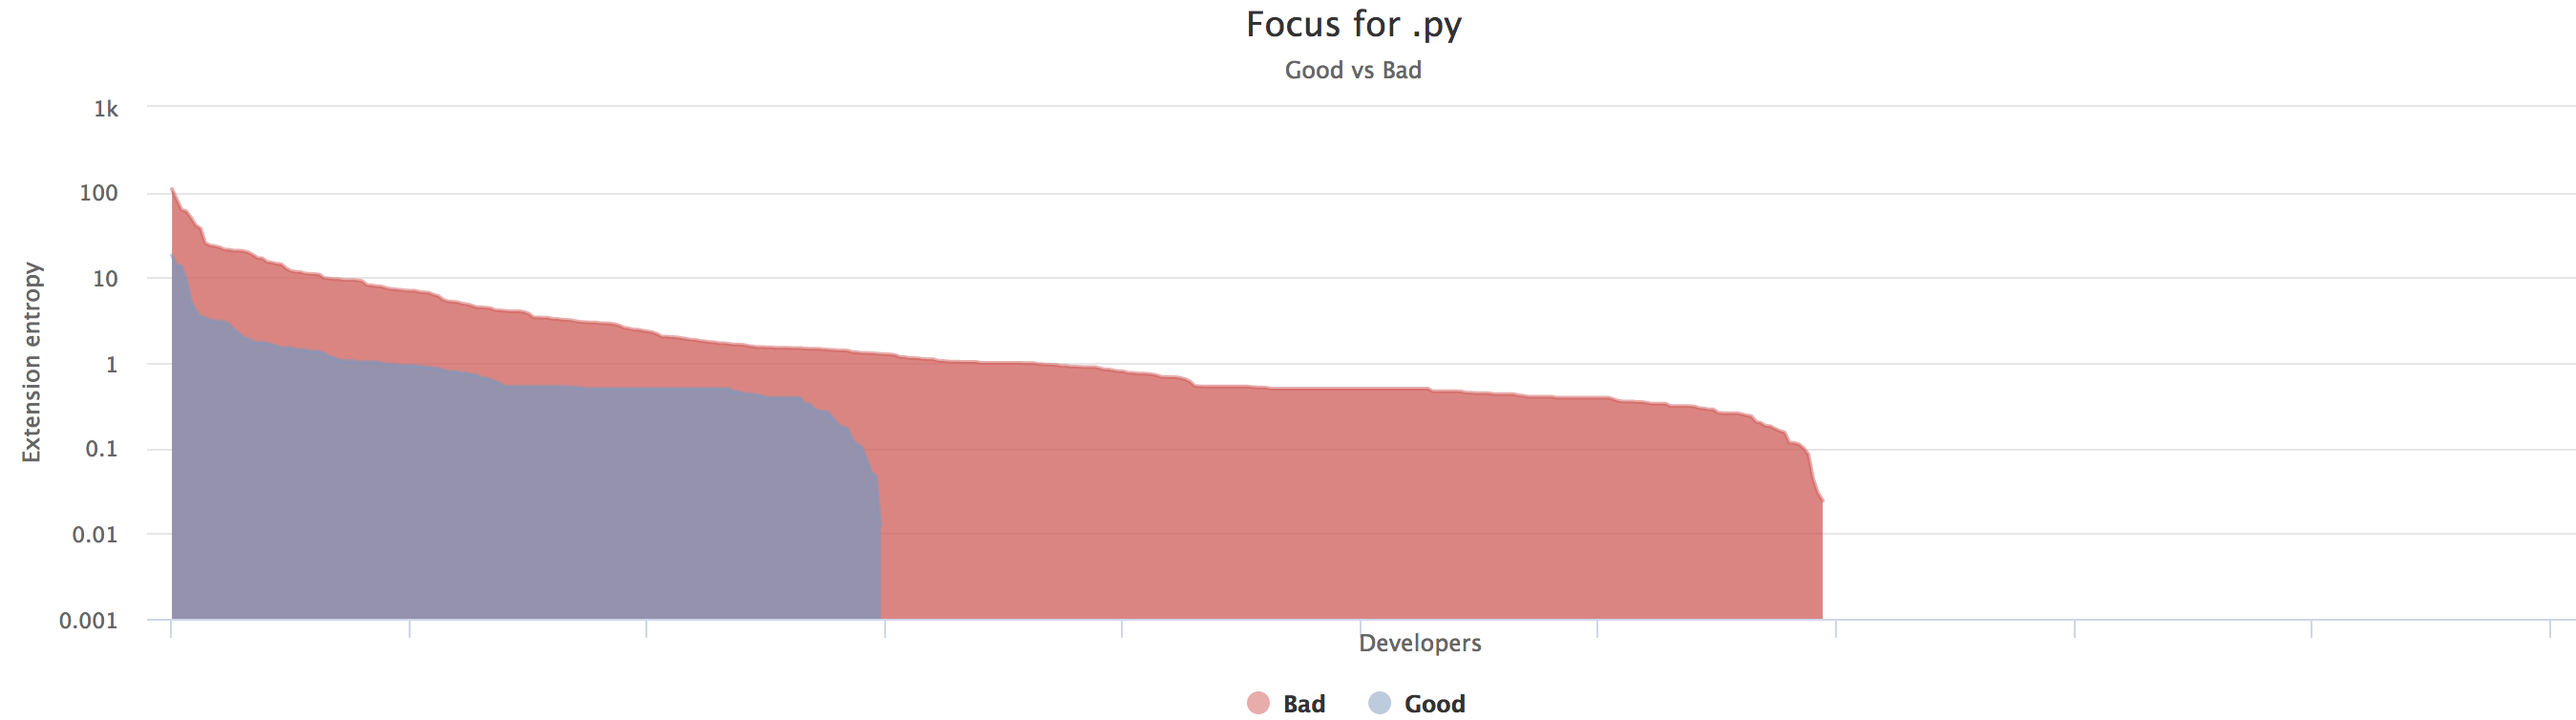
\includegraphics[width=1\textwidth]{figures/py_log}
  \caption[Focus Chart for .py]{Clearly \textit{good developers} focus more on .py extensions since the entropy levels are lower. This chart also shows that there are more \textit{bad developers} working on this extension.} \label{fig:py_log_appendix}
\end{figure}

\begin{figure}[htpb]
  \centering
  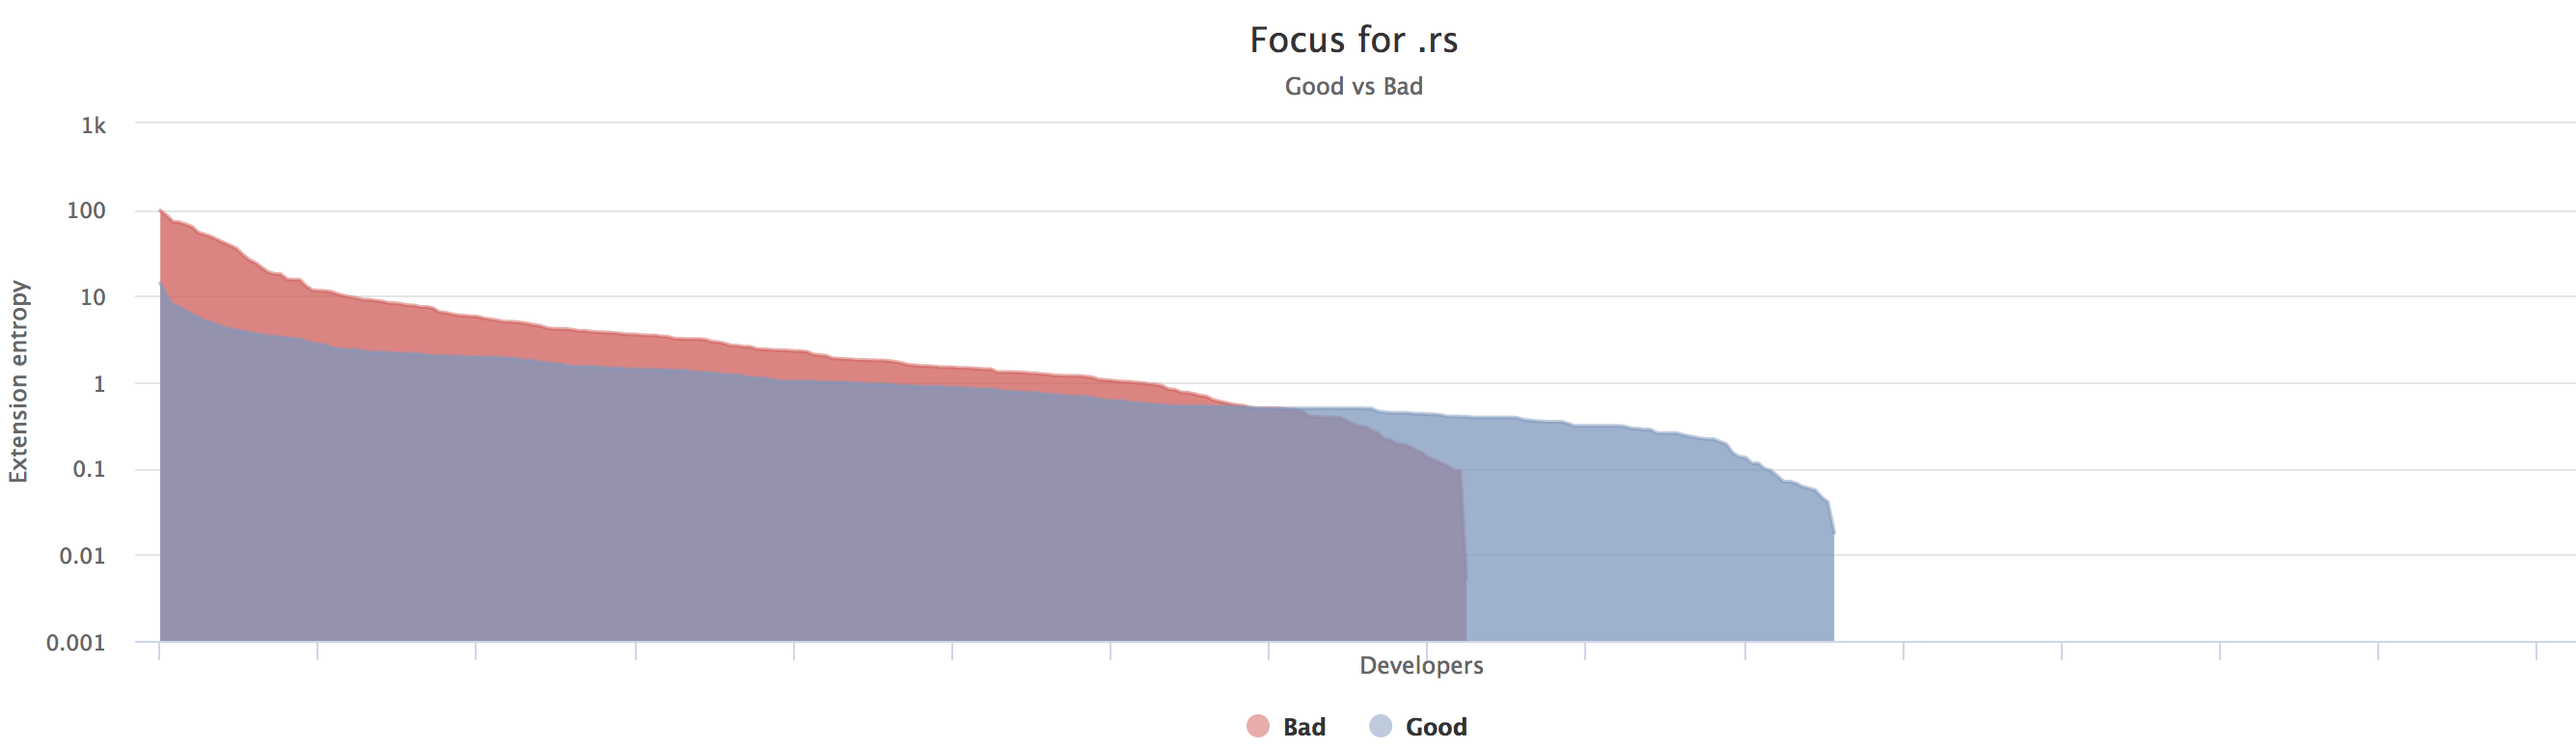
\includegraphics[width=1\textwidth]{figures/rs_log}
  \caption[Focus Chart for .rs]{Clearly \textit{good developers} focus more on .rs extensions since the entropy levels are lower. This chart also shows that there are more \textit{good developers} working on this extension.} \label{fig:rs_log_appendix}
\end{figure}

\begin{figure}[htpb]
  \centering
  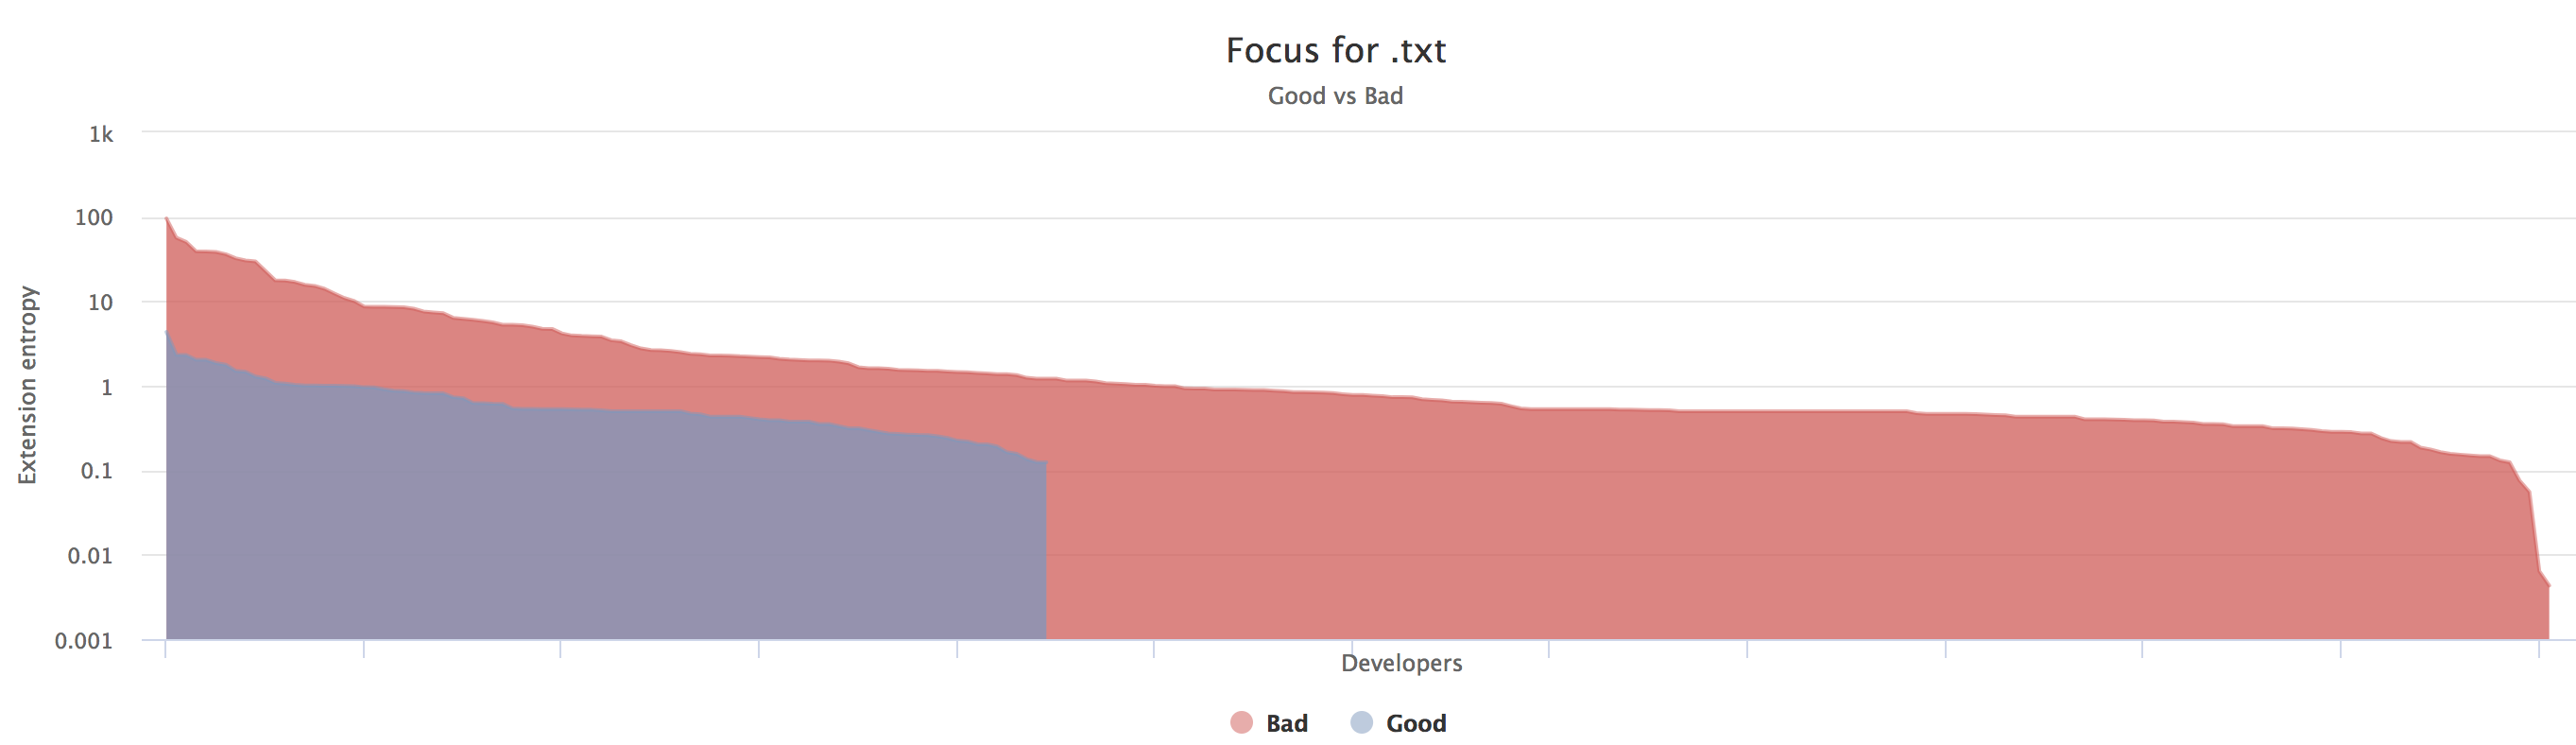
\includegraphics[width=1\textwidth]{figures/txt_log}
  \caption[Focus Chart for .txt]{Clearly \textit{good developers} focus more on .txt extensions since the entropy levels are lower. This chart also shows that there are more \textit{bad developers} working on this extension.} \label{fig:txt_log_appendix}
\end{figure}

\begin{figure}[htpb]
  \centering
  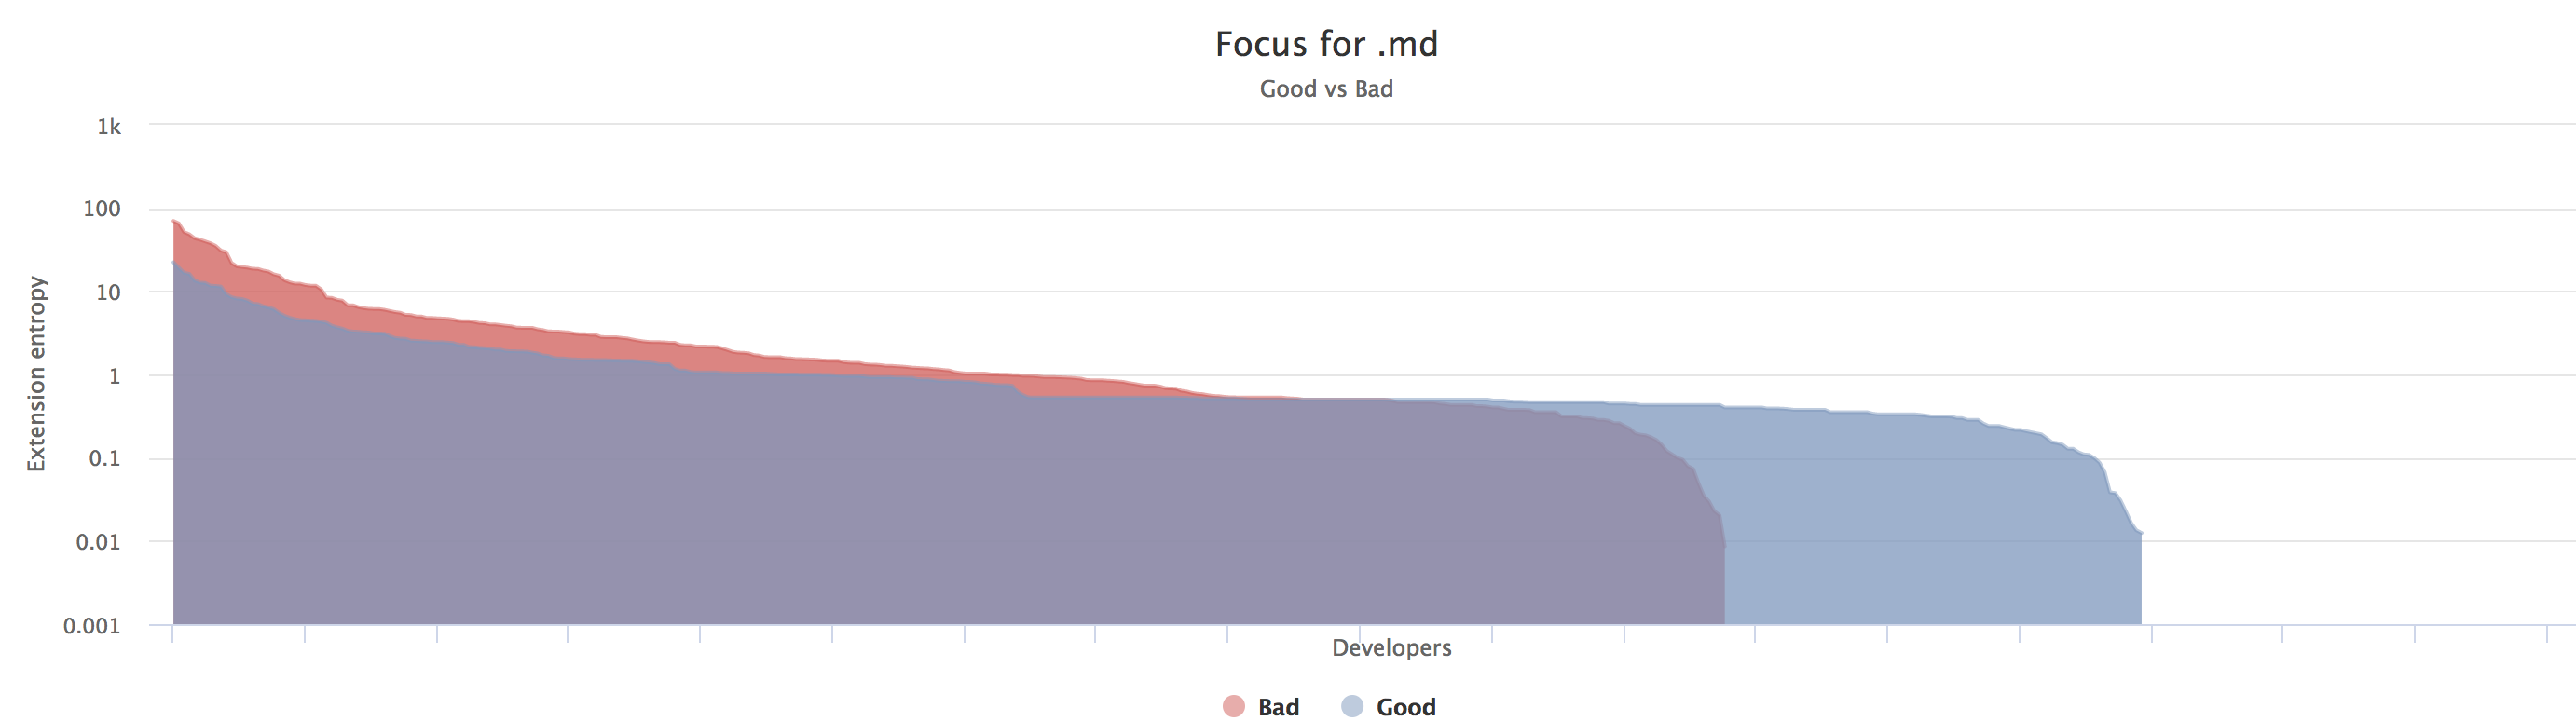
\includegraphics[width=1\textwidth]{figures/md_log}
  \caption[Focus Chart for .md]{Clearly \textit{good developers} focus more on .md extensions since the entropy levels are lower. This chart also shows that there are more \textit{good developers} working on this extension.} \label{fig:md_log_appendix}
\end{figure}

\begin{figure}[htpb]
  \centering
  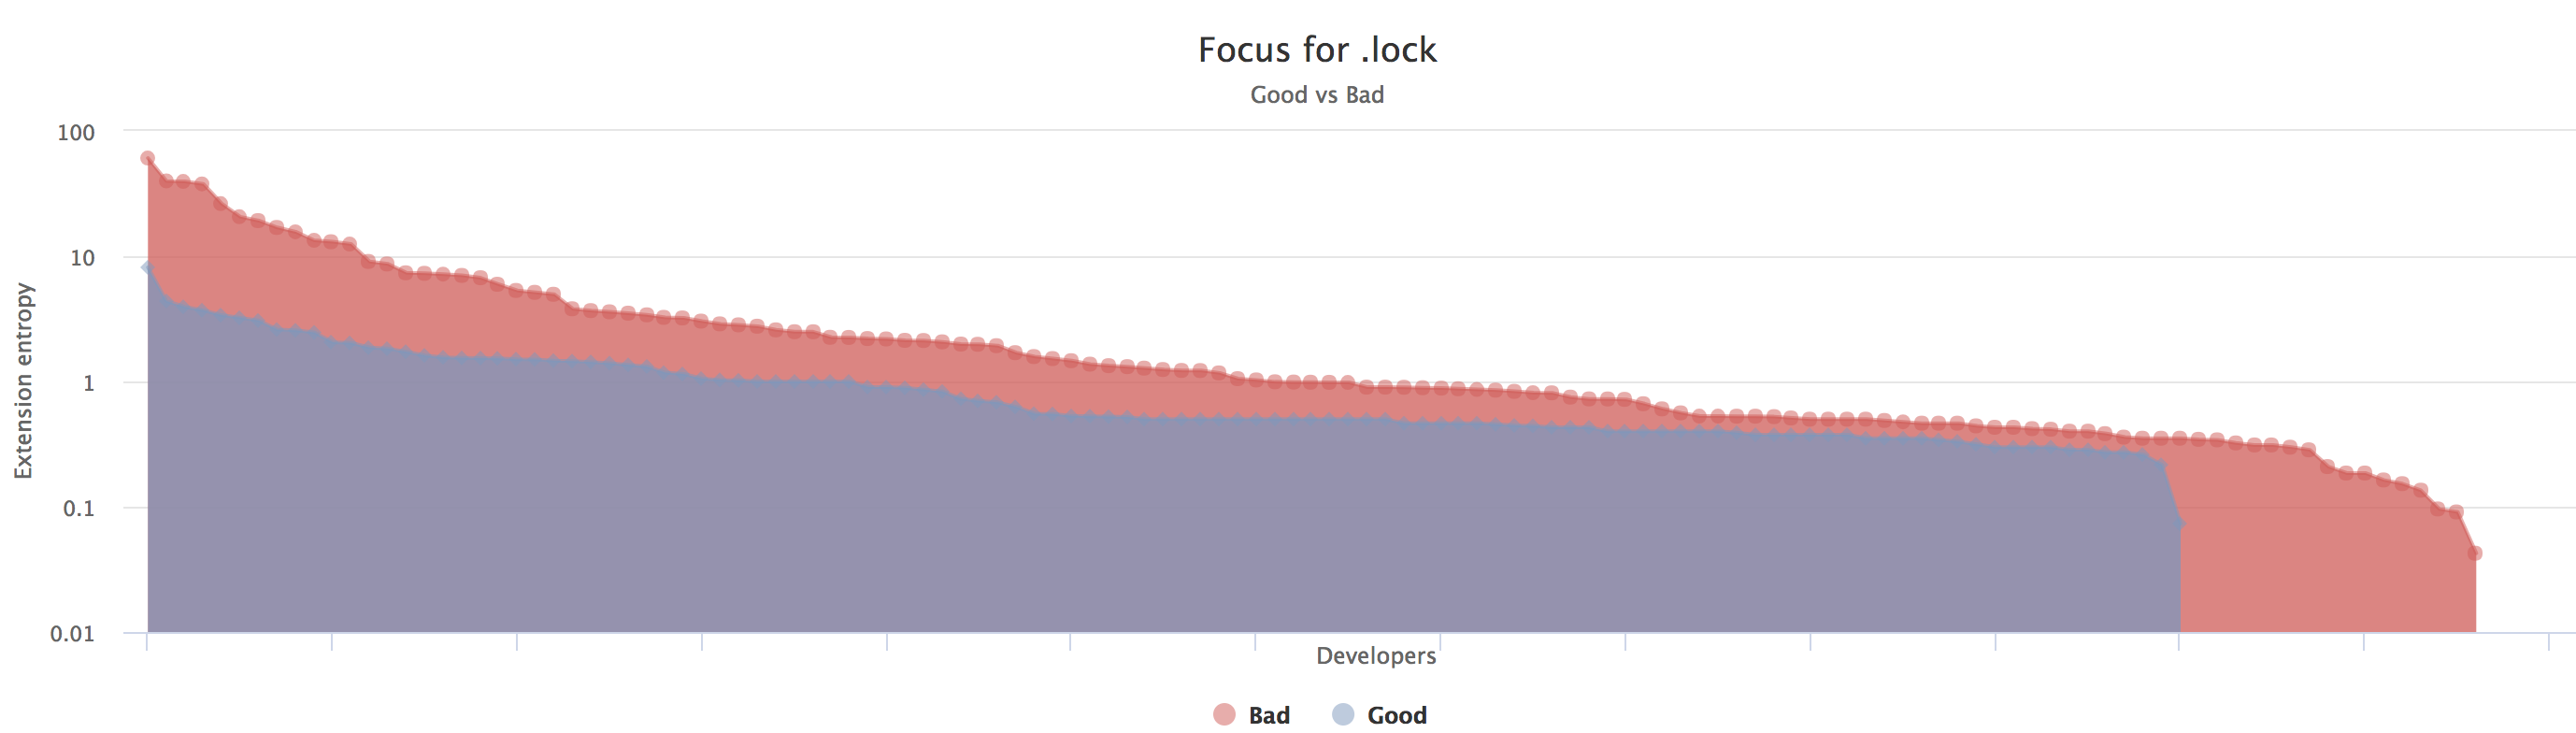
\includegraphics[width=1\textwidth]{figures/lock_log}
  \caption[Focus Chart for .lock]{This chart is displayed because .lock is one of the ten most popular extensions. However since developers do not directly modify it, it is not discussed.} \label{fig:lock_log_appendix}
\end{figure}

\begin{figure}[htpb]
  \centering
  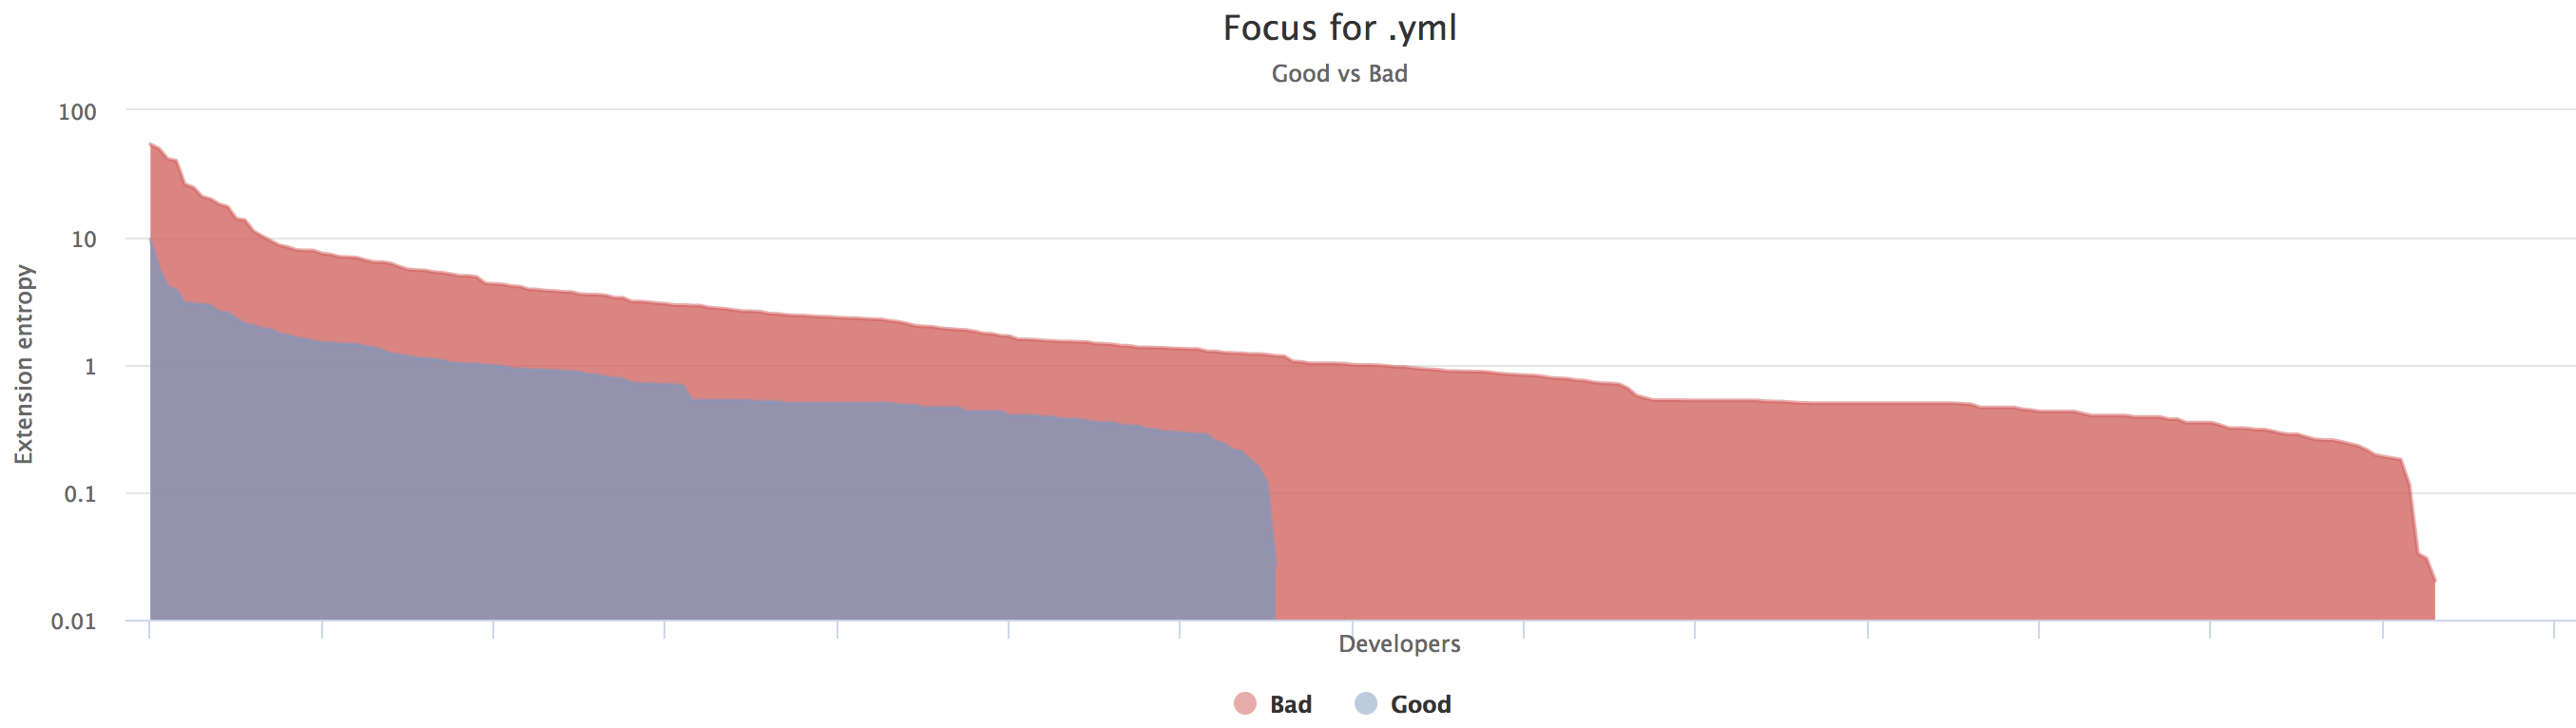
\includegraphics[width=1\textwidth]{figures/yml_log}
  \caption[Focus Chart for .yml]{Clearly \textit{good developers} focus more on .yml extensions since the entropy levels are lower. This chart also shows that there are more \textit{bad developers} working on this extension.} \label{fig:yml_log_appendix}
\end{figure}

\begin{figure}[htpb]
  \centering
  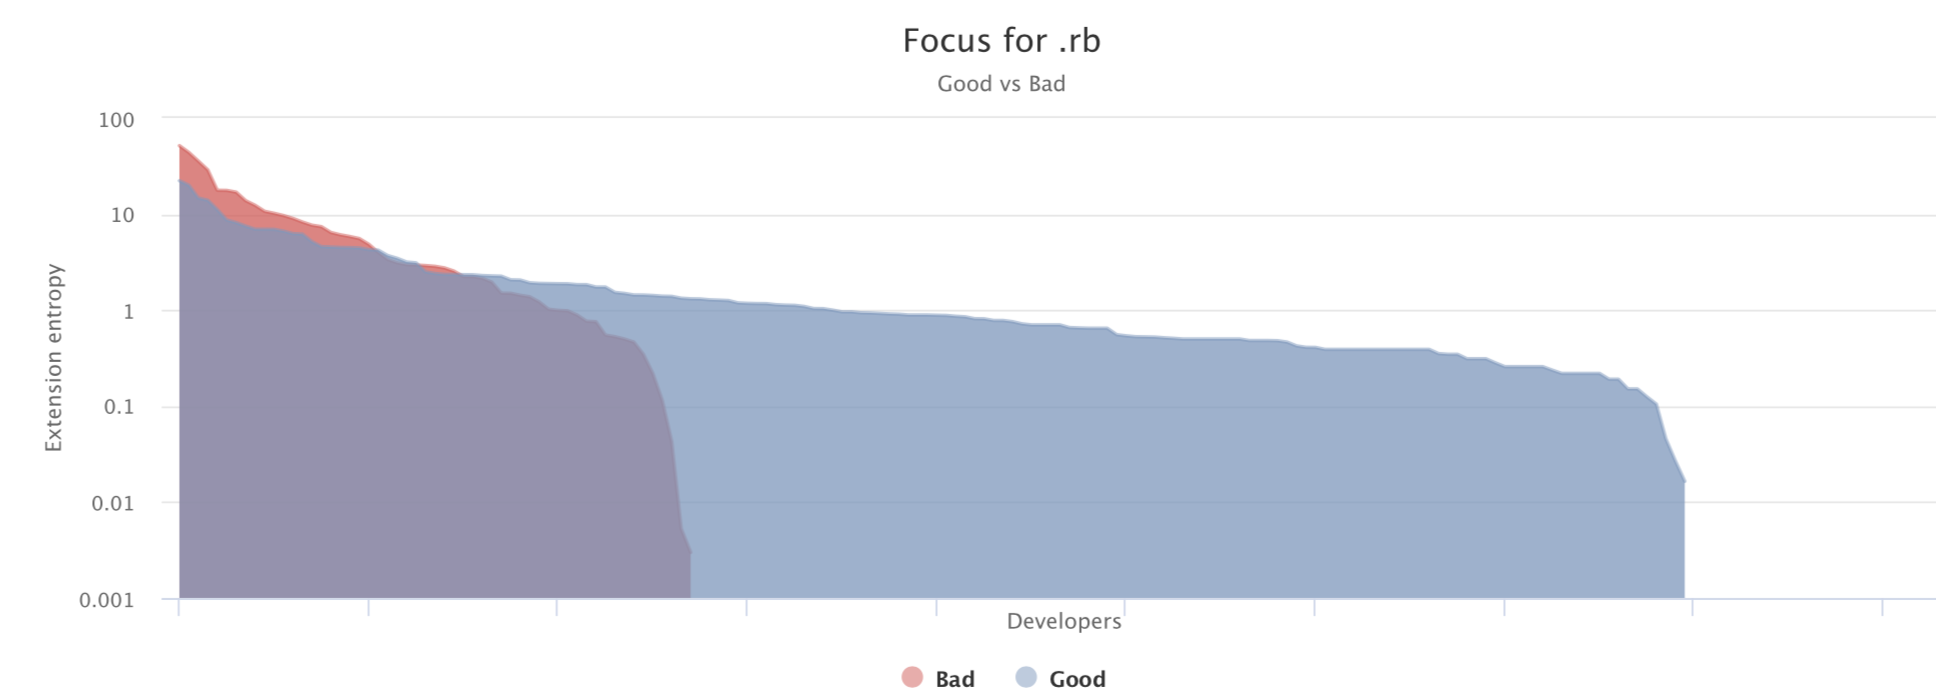
\includegraphics[width=1\textwidth]{figures/rb_log}
  \caption[Focus Chart for .rb]{Both groups of developers focus on .rb extensions in a similar way. This chart also shows that there are more \textit{good developers} working on this extension.} \label{fig:rb_log_appendix}
\end{figure}



% \chapter{Figures}
% \section{Example 1}
% \cmark
% \section{Example 2}
% \xmark